\documentclass{article}

%Preamble
\title{CS 585 Assignment 2}
\author{Don Johnson}
\date{January 29, 2014}
\usepackage{graphicx}
\usepackage[margin=0.5in]{geometry}
\usepackage{listings}
\lstset{language=C}
\usepackage{caption}
\usepackage{subcaption}
\usepackage{underscore}
\usepackage{mathtools}
\usepackage{float}

%Content
\begin{document}
\maketitle
\section{Assignment 2 (100 points)}
\subsection{Learning Objectives}
\subsection{Technical Task (30 points)}
Source code for technical task in ZIP file: Assignment2.cpp, Assignment2.hpp, Gui.cpp and Operators.cpp. All output images are in a subfolder in the ZIP file called "assignment2/Data."

\subsection{Programming Assignment Questions (28 points)}

\begin{enumerate}

\item
Run your program on the image yellowEgg.jpg both by thresholding the gradient magnitude and by using the Canny edge detector. Choose a threshold and smoothing level that leads to a nice contour and filled region of the egg. Results below:

Note: Smoothing value units are one standard deviation and threshold values are pixel integer values. Unlike the gradient edge detector, the Canny has both a lower and upper threshold that I set to be threes times the lower threshold. Consequently, the Canny output files have two thresholds in their name.

\begin{figure}[!htbp]
\centering
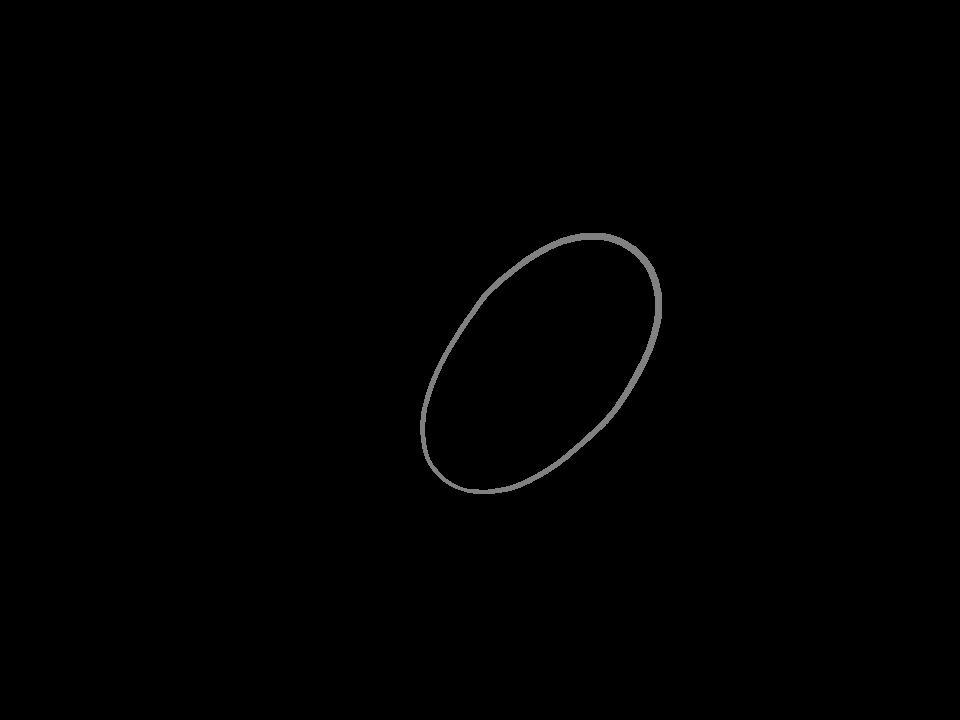
\includegraphics[width=140mm]{/Users/donj/workspace/cs585/Lab2/Mac/Assignment2/Data/SoloYellowEgg-Gradient-edges-2pt5-82.png}
\caption{SoloYellowEgg-Gradient-edges-2pt5-82.png}
\label{overflow}
\end{figure}

\begin{figure}[H]
\centering
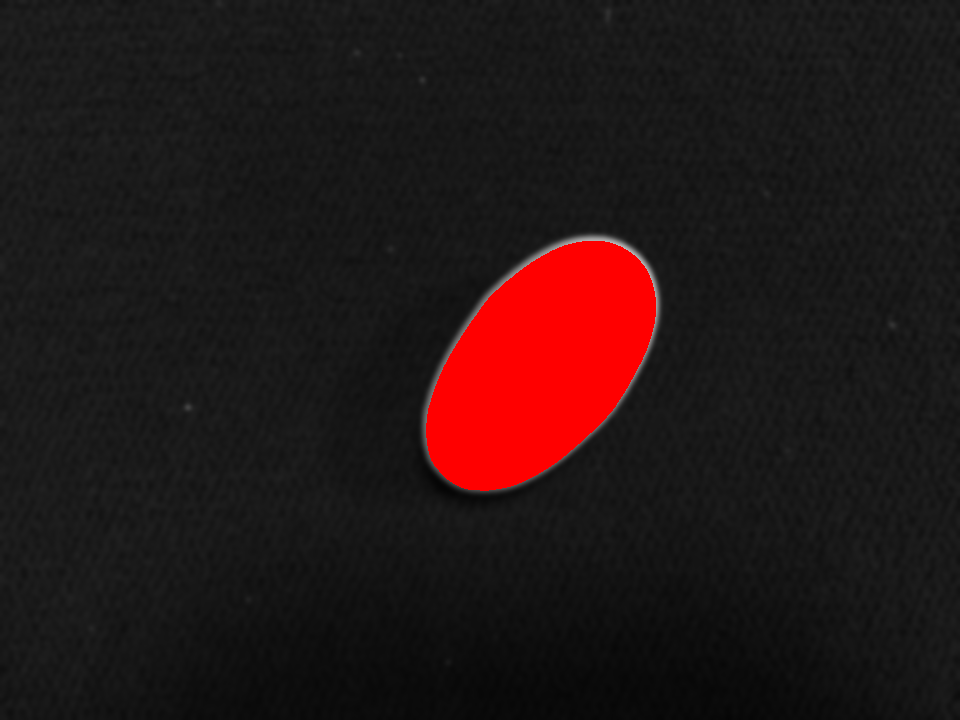
\includegraphics[width=140mm]{/Users/donj/workspace/cs585/Lab2/Mac/Assignment2/Data/SoloYellowEgg-Gradient-result-2pt5-82.png}
\caption{SoloYellowEgg-Gradient-result-2pt5-82.png}
\label{overflow}
\end{figure}

\begin{figure}[H]
\centering
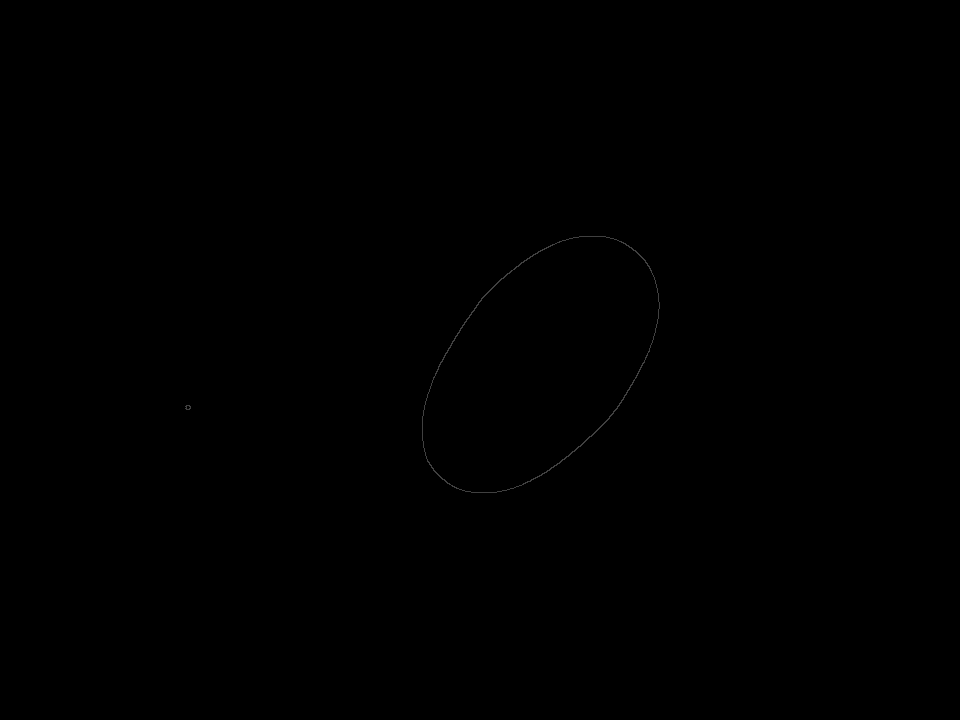
\includegraphics[width=140mm]{/Users/donj/workspace/cs585/Lab2/Mac/Assignment2/Data/SoloYellowEgg-Canny-edges-1-129-387.png}
\caption{SoloYellowEgg-Canny-edges-1-129-387.png}
\label{overflow}
\end{figure}

\begin{figure}[H]
\centering
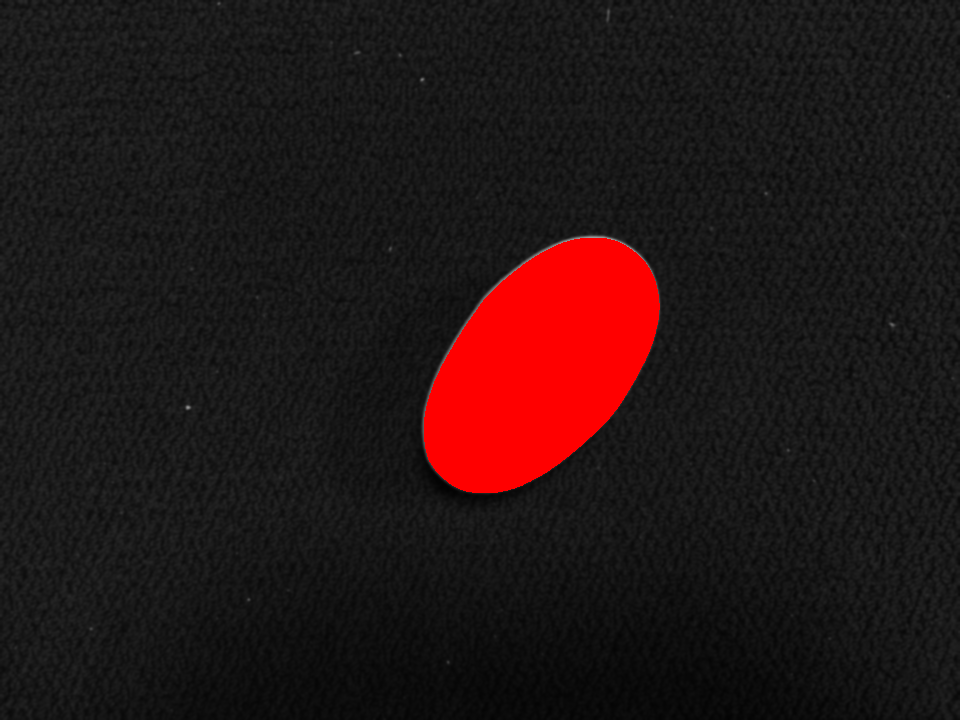
\includegraphics[width=140mm]{/Users/donj/workspace/cs585/Lab2/Mac/Assignment2/Data/SoloYellowEgg-Canny-result-1-129-387.png}
\caption{SoloYellowEgg-Canny-result-1-129-387.png}
\label{overflow}
\end{figure}

\item
Run your program on the image "eggsAndCube.jpg." Choose a smoothing level that you feel gives good contours in the gradient magnitude, and then for each of the red, green, blue, and yellow eggs, choose the highest threshold that gives a clean result. Results below:

\begin{figure}[H]
\centering
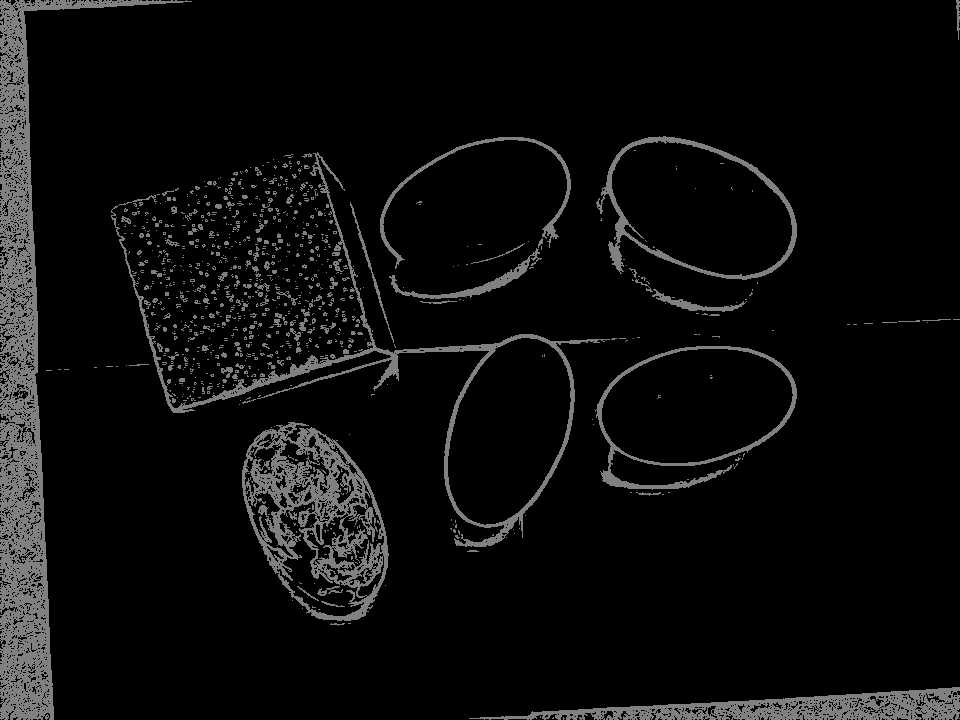
\includegraphics[width=140mm]{/Users/donj/workspace/cs585/Lab2/Mac/Assignment2/Data/redEgg-edges-0pt5-41.png}
\caption{redEgg-edges-0pt5-41.png}
\label{overflow}
\end{figure}

\begin{figure}[H]
\centering
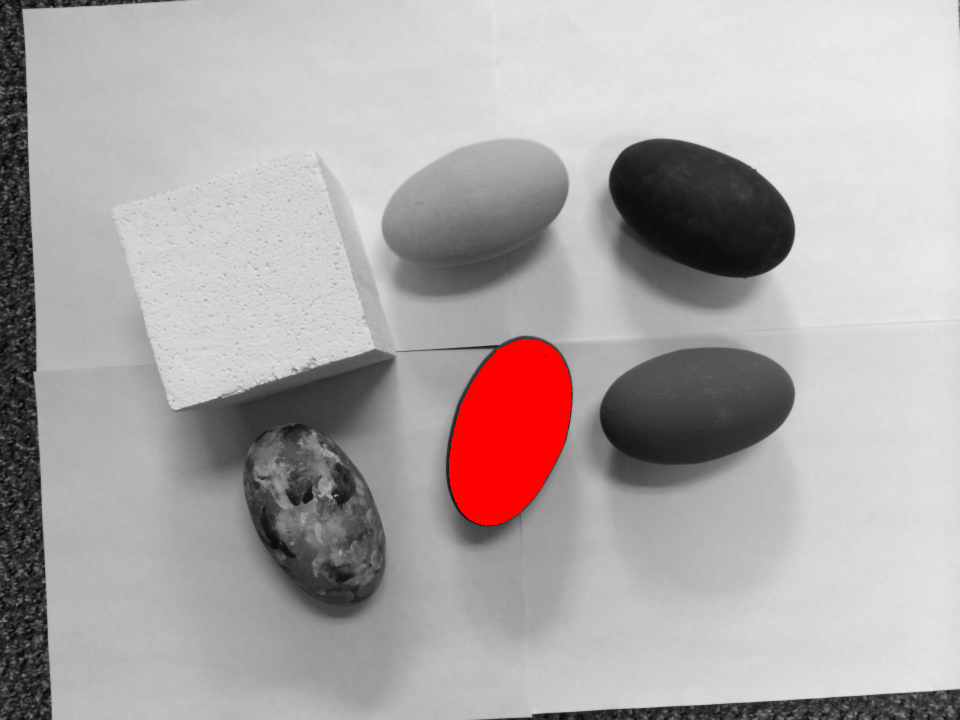
\includegraphics[width=140mm]{/Users/donj/workspace/cs585/Lab2/Mac/Assignment2/Data/redEgg-result-0pt5-41.png}
\caption{redEgg-result-0pt5-41.png}
\label{overflow}
\end{figure}

\begin{figure}[H]
\centering
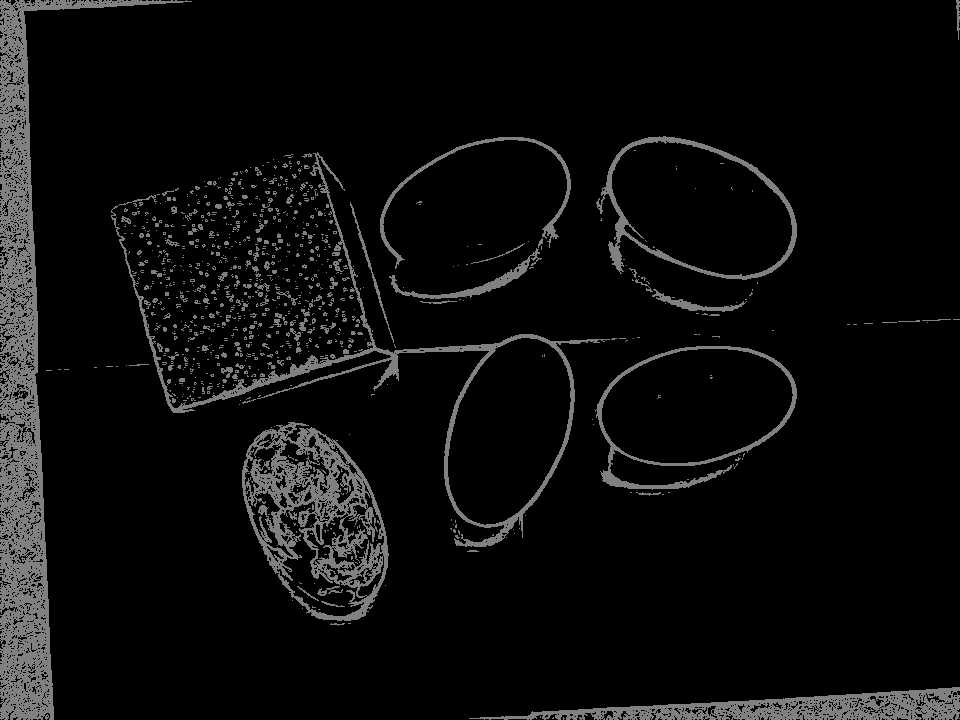
\includegraphics[width=140mm]{/Users/donj/workspace/cs585/Lab2/Mac/Assignment2/Data/greenEgg-edges-0pt5-41.png}
\caption{greenEgg-edges-0pt5-41.png}
\label{overflow}
\end{figure}

\begin{figure}[H]
\centering
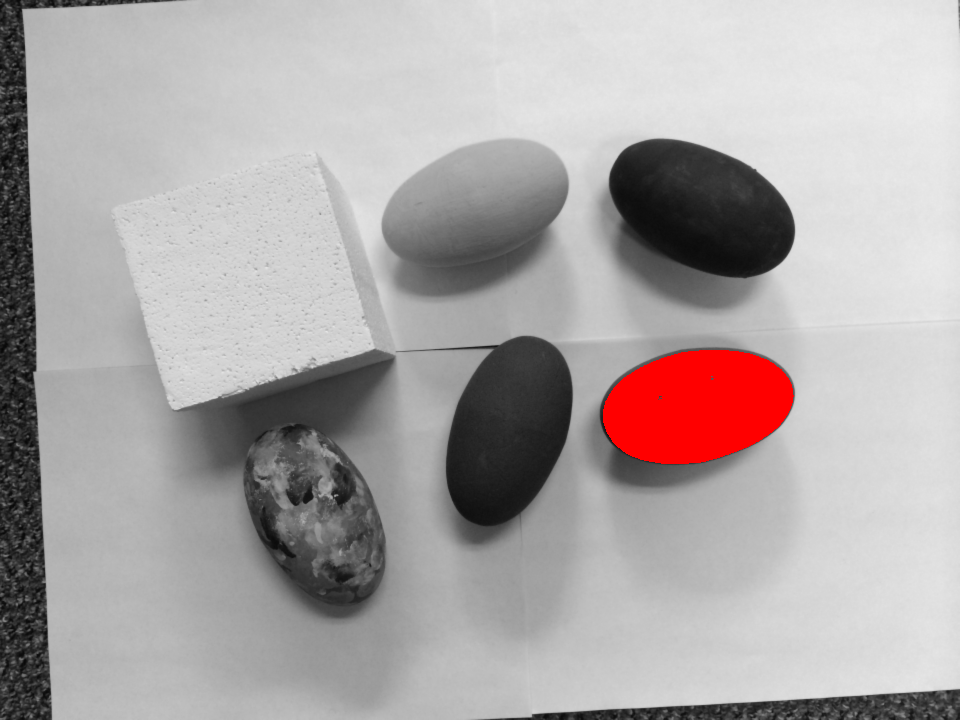
\includegraphics[width=140mm]{/Users/donj/workspace/cs585/Lab2/Mac/Assignment2/Data/greenEgg-result-0pt5-41.png}
\caption{greenEgg-result-0pt5-41.png}
\label{overflow}
\end{figure}

\begin{figure}[H]
\centering
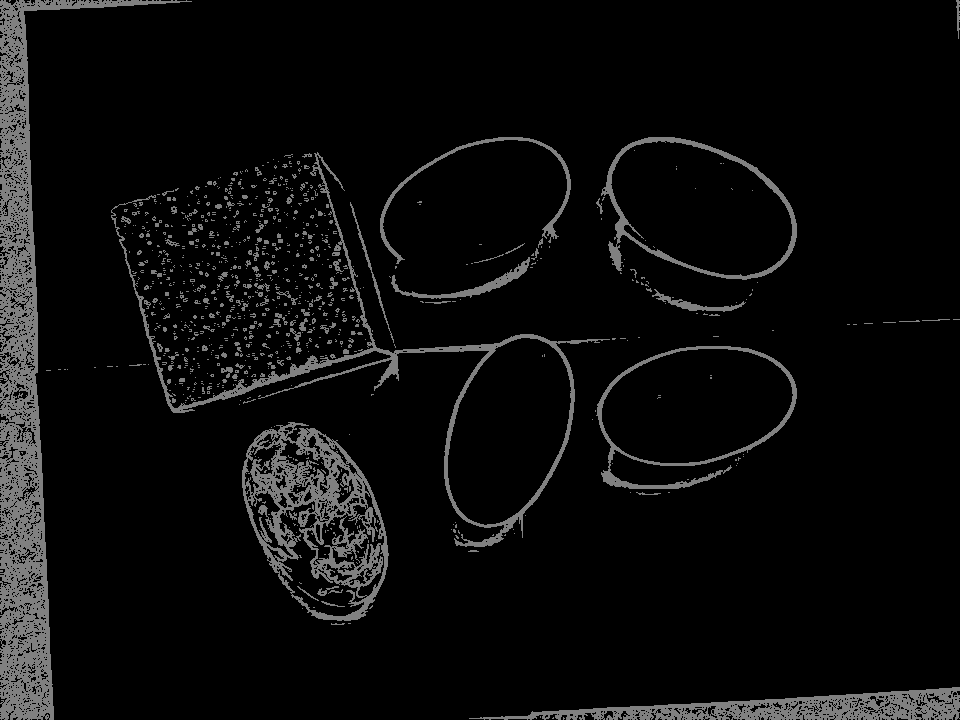
\includegraphics[width=140mm]{/Users/donj/workspace/cs585/Lab2/Mac/Assignment2/Data/blueEgg-edges-0pt5-42.png}
\caption{blueEgg-edges-0pt5-42.png}
\label{overflow}
\end{figure}

\begin{figure}[H]
\centering
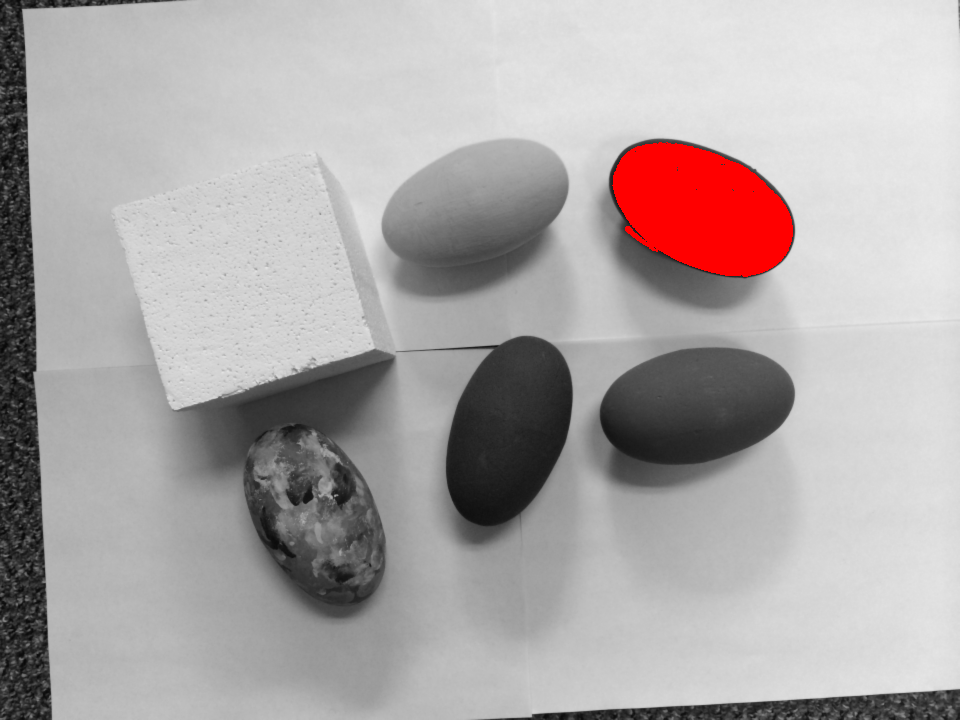
\includegraphics[width=140mm]{/Users/donj/workspace/cs585/Lab2/Mac/Assignment2/Data/blueEgg-result-0pt5-42.png}
\caption{blueEgg-result-0pt5-42.png}
\label{overflow}
\end{figure}

\item
Are you able to find any parameters that will allow you to identify the cube (or a face of the cube)? 

Harder with "gradient," because of the texture of the cube. Need low threshold and higher smoothing, however with "Canny" with dilation it is easy to select the same face on the cube cleanly (Smoothing sigma = 1.5, Canny thresholds = 20 and 60, Dilation kernel size = 3). See the results below (right vertical face):

\begin{figure}[H]
\centering
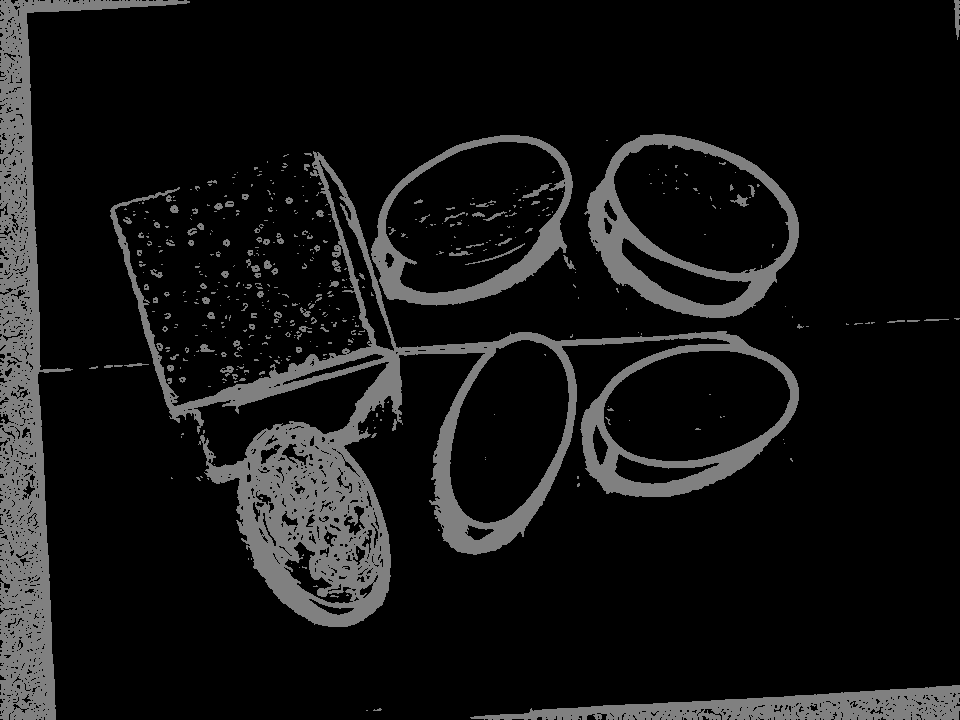
\includegraphics[width=140mm]{/Users/donj/workspace/cs585/Lab2/Mac/Assignment2/Data/cube-edges-1pt5-16.png}
\caption{cube-edges-1pt5-16.png}
\label{overflow}
\end{figure}

\begin{figure}[H]
\centering
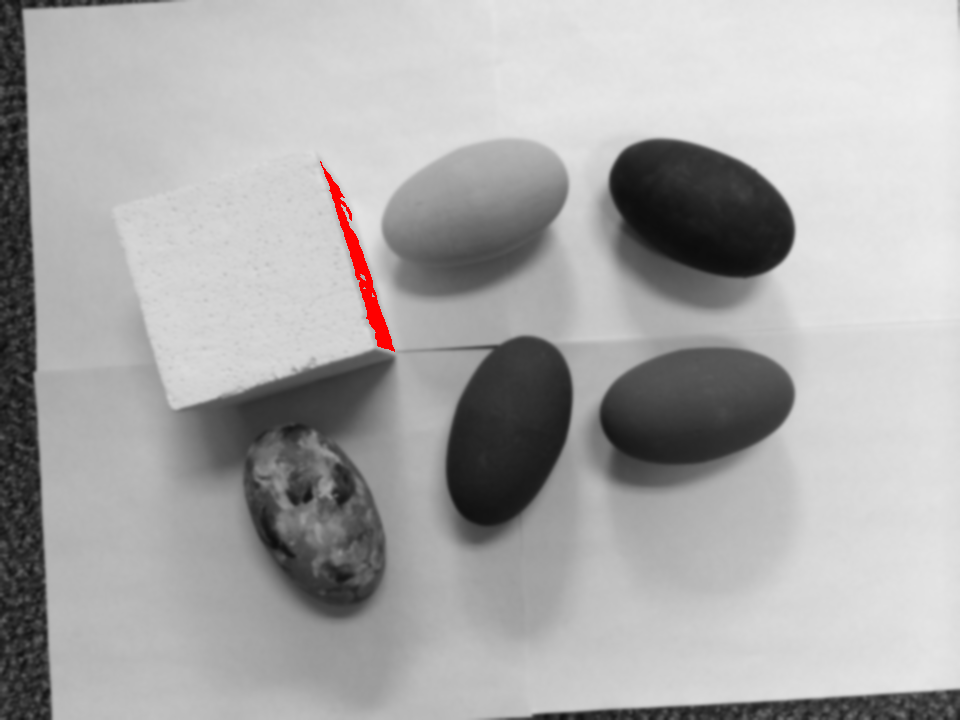
\includegraphics[width=140mm]{/Users/donj/workspace/cs585/Lab2/Mac/Assignment2/Data/cube-result-1pt5-16.png}
\caption{cube-result-1pt5-16.png}
\label{overflow}
\end{figure}

\begin{figure}[H]
\centering
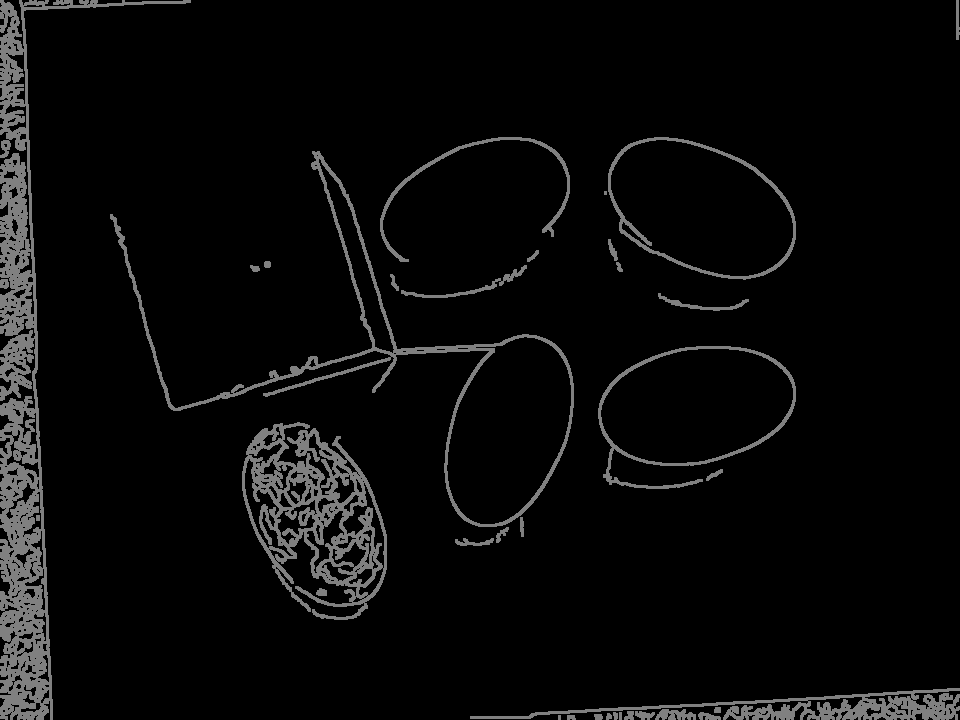
\includegraphics[width=140mm]{/Users/donj/workspace/cs585/Lab2/Mac/Assignment2/Data/cube-canny-dilation-edges.png}
\caption{cube-canny-dilation-edges.png}
\label{overflow}
\end{figure}

\begin{figure}[H]
\centering
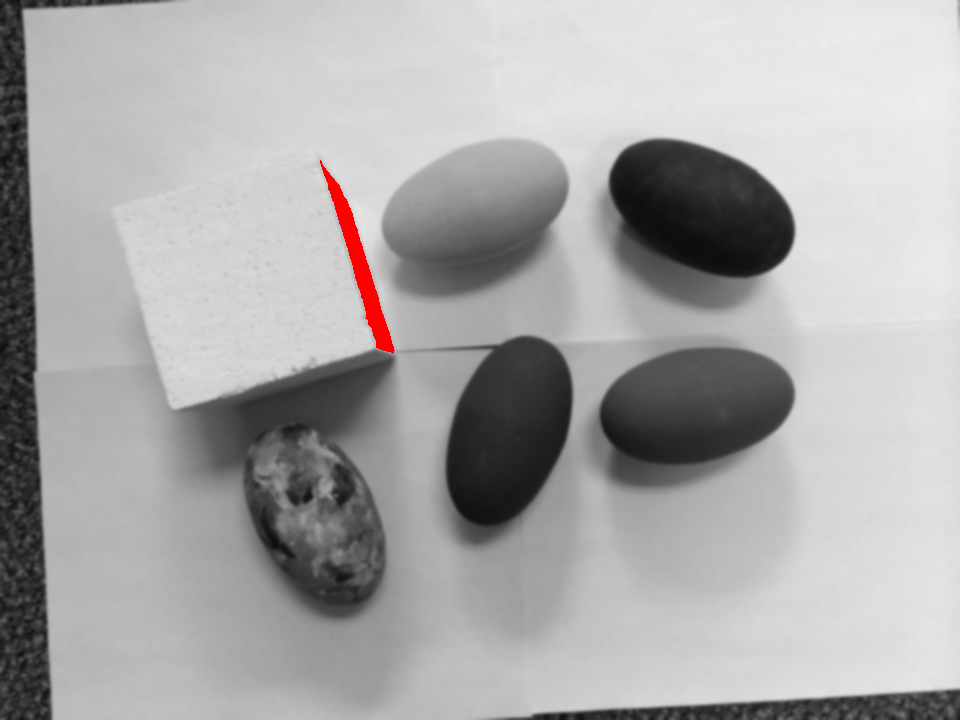
\includegraphics[width=140mm]{/Users/donj/workspace/cs585/Lab2/Mac/Assignment2/Data/cube-canny-dilation-result.png}
\caption{cube-canny-dilation-result.png}
\label{overflow}
\end{figure}

\pagebreak
\item
Use your program on the image "camoEggsOnPaper.jpg." If you knew that you were looking for textured objects on a plain background, what steps could you combine in order to highlight an entire egg, even though there are lots of internal edges? What type of binary image analysis steps could you perform in order to segment the entire egg? 

Canny with high thresholds (low=149 and high=447) and 3x3 kernel dilation can the closest to working. Nothing I tried to close off the eggs edges without almost filling the eggs with mask. Initial smoothing wasn't needed and didn't help for Canny, because Canny does a Gaussian smoothing as part of its procedure. Results below:

\begin{figure}[H]
\centering
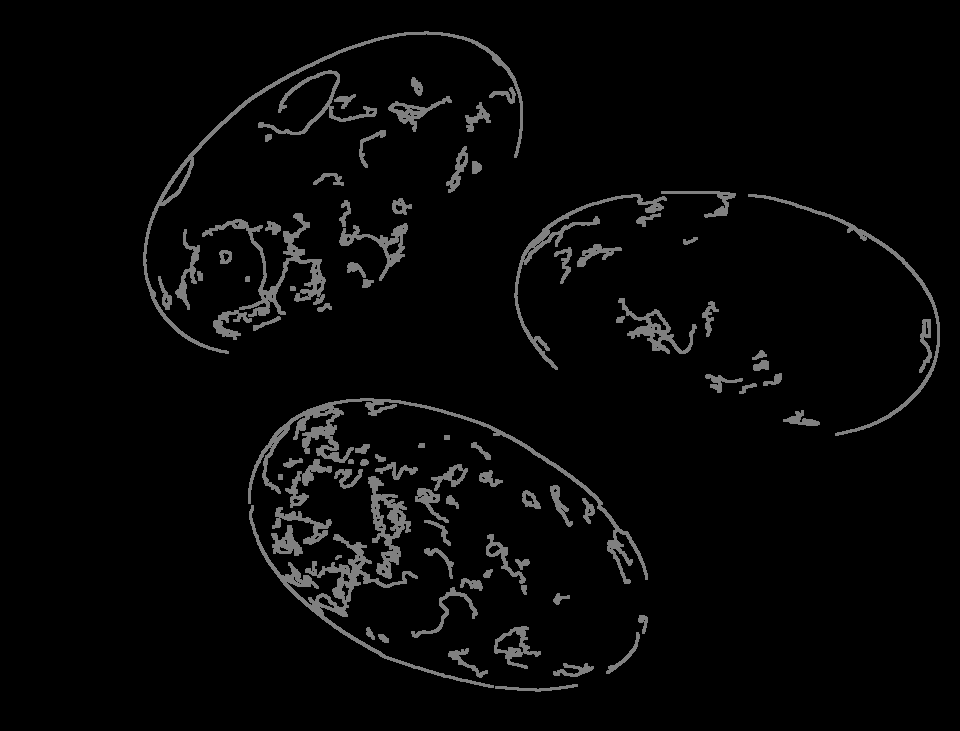
\includegraphics[width=140mm]{/Users/donj/workspace/cs585/Lab2/Mac/Assignment2/Data/camoEggsOnPaper-canny-dilation-edges.png}
\caption{camoEggsOnPaper-canny-dilation-edges.png}
\label{overflow}
\end{figure}


\item
Run your program on the image rainbowSpheres.jpg. You may find that some areas of the image are easier to segment than others. Try clicking on a few image regions (spots or stripes on the balls). Results below:

\begin{figure}[H]
\centering
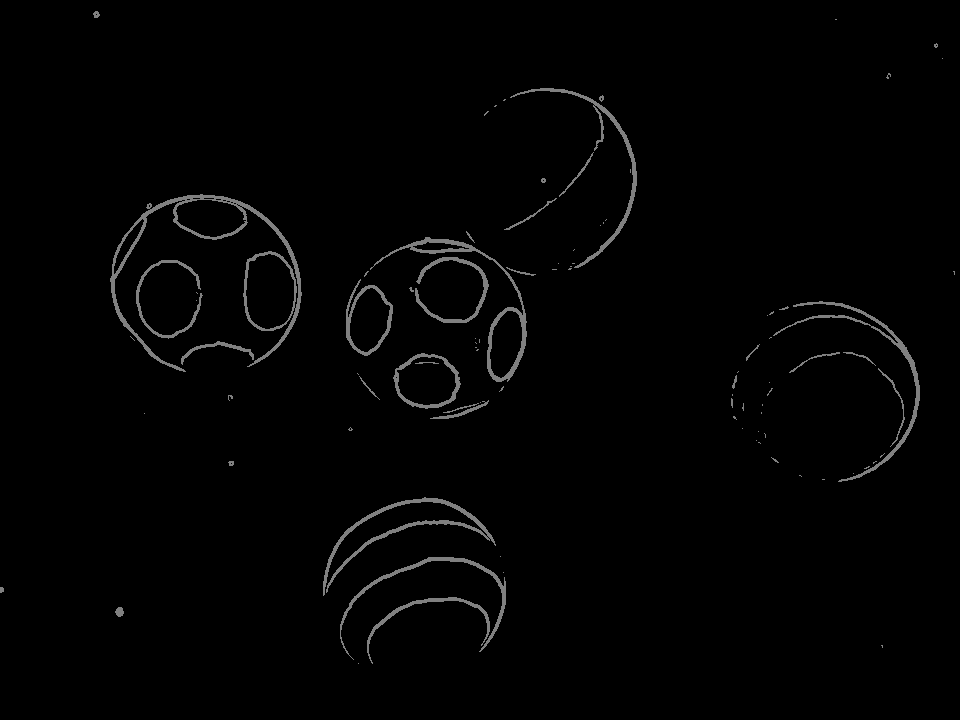
\includegraphics[width=140mm]{/Users/donj/workspace/cs585/Lab2/Mac/Assignment2/Data/rainbowEasy-edges-1-94.png}
\caption{rainbowEasy-edges-1-94.png}
\label{overflow}
\end{figure}

\begin{figure}[H]
\centering
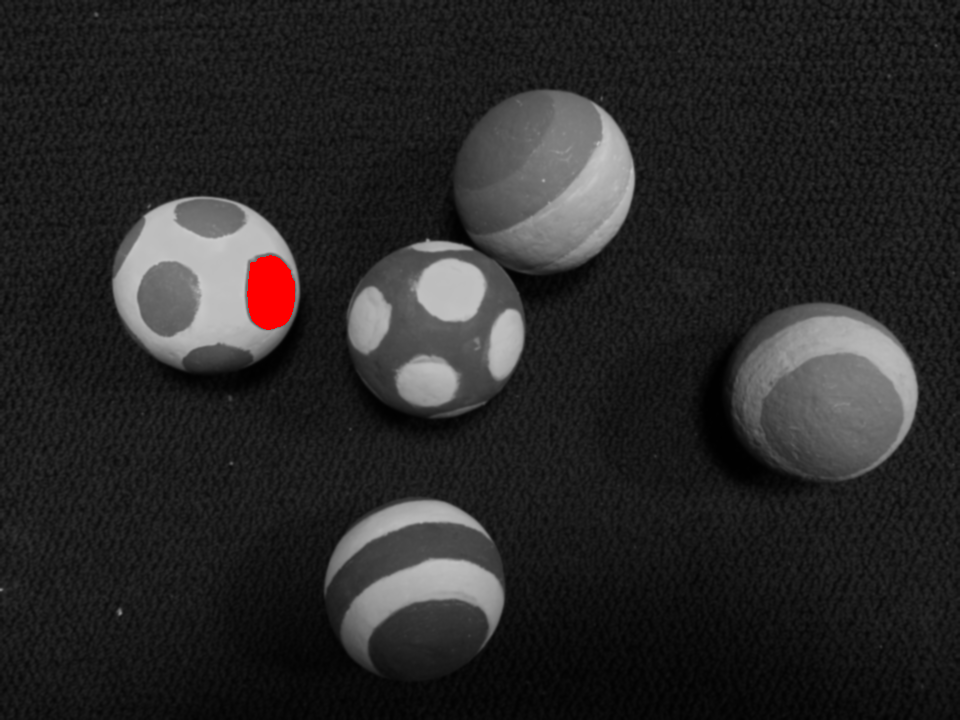
\includegraphics[width=140mm]{/Users/donj/workspace/cs585/Lab2/Mac/Assignment2/Data/rainbowEasy-result-1-94.png}
\caption{rainbowEasy-result-1-94.png}
\label{overflow}
\end{figure}


\item
Identify an area of the image that you think should be reasonably easy to pick out, but that the program is having trouble with. (For example, the purple and blue stripes on top of the rainbow ball). What is happening that causes the entire background to be filled when you attempt to fill the region bounded by edges starting in one of these areas?

The entire background is filled because the strip I picked out was missing part of its left edge.

\item
Use morphological operators to manipulate your edge map to help close gaps where the region-filling is leaking out so that you can fill in difficult region. Create before and after images of your troublesome regions. 

I used 1 sigma smoothing, a lower threshold and  a 3x3 kernel dilation to fill the gap. Results below:

\begin{figure}[H]
\centering
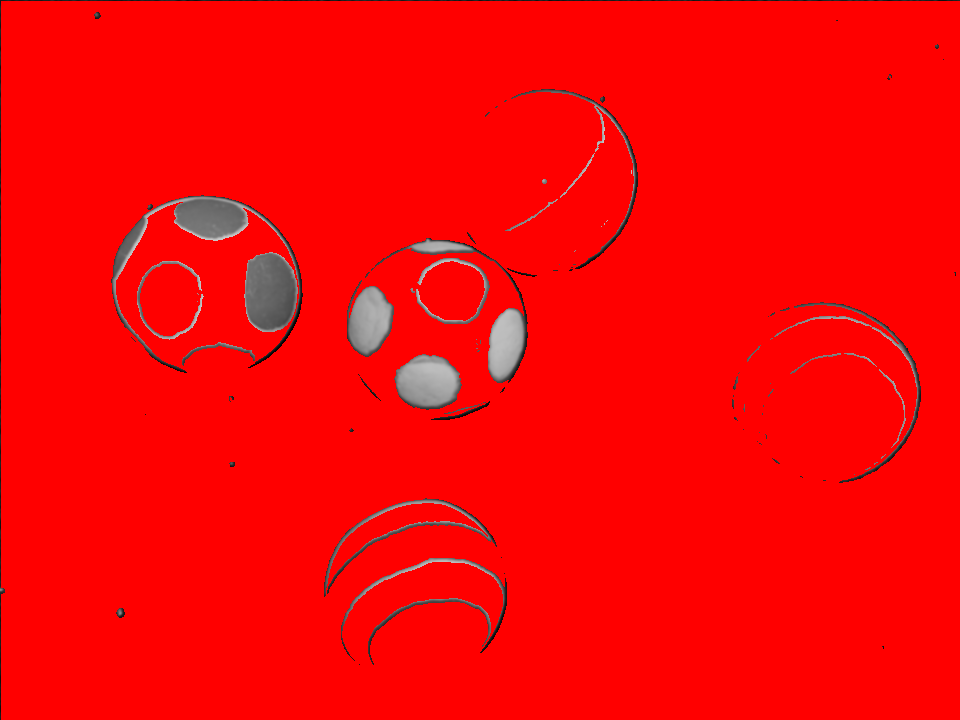
\includegraphics[width=140mm]{/Users/donj/workspace/cs585/Lab2/Mac/Assignment2/Data/rainbowHard-before-result-1-94.png}
\caption{rainbowHard-before-result-1-94.png}
\label{overflow}
\end{figure}

\begin{figure}[H]
\centering
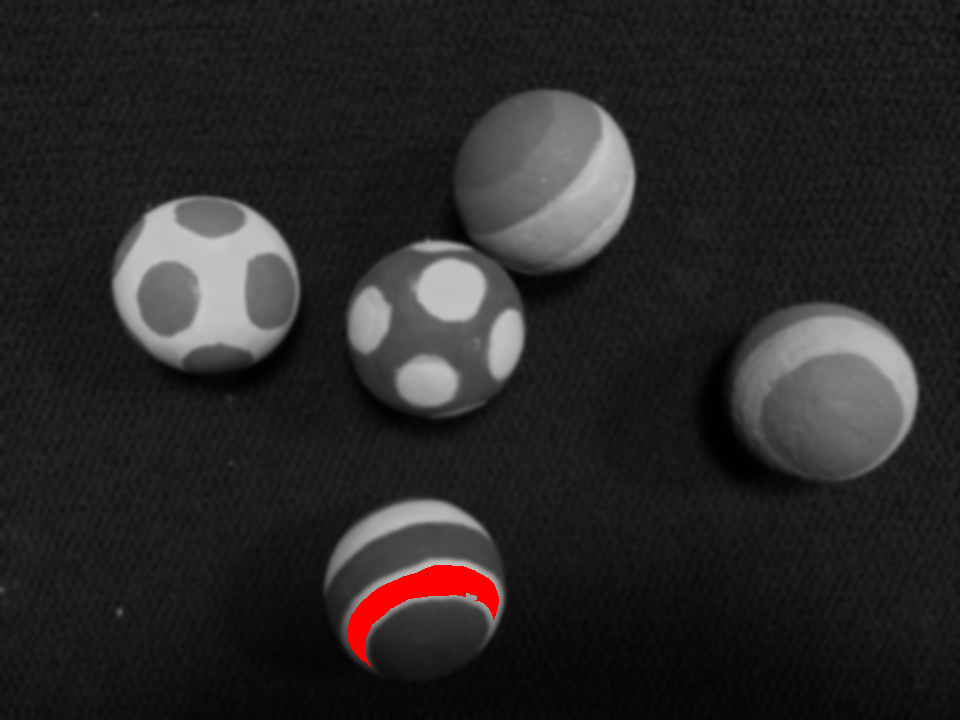
\includegraphics[width=140mm]{/Users/donj/workspace/cs585/Lab2/Mac/Assignment2/Data/rainbowHard-after-result-1-33.png}
\caption{rainbowHard-after-result-1-33.png}
;\label{overflow}
;\end{figure}

\end{enumerate}

\subsection{Lab Follow-up Questions (39 points)}
\begin{enumerate}

\item
Under the folder for Lab2, there is a folder called "gradients" containing several image where I have prepared several images using the gradient formula. Remember that the gradient of a function is just a vector containing the partial derivatives of the function with respect to each variable. You take a partial derivative of a function using the normal rules of calculus, but you treat all variables other than the one you are interested in as constants.


  \begin{enumerate}
    \item Write an expression for the gradient of I, given the formula that I used to generate the images.
    
    Holding y, \(\theta\) constant and taking the derivative with respect to x yields:
    
\begin{eqnarray*}
\frac{\partial I}{\partial x} I(x,y)=\cos \theta
\end{eqnarray*}    
    
        Holding x, \(\theta\)  constant and taking the derivative with respect to y yields:
    
\begin{eqnarray*}
\frac{\partial I}{\partial y} I(x,y)=\sin \theta
\end{eqnarray*}    

    \item For each of three values calculate what you anticipate the values of the gradient will be:
\begin{eqnarray*}
\nabla I \left( \theta \right)=\left( \sin \theta, \cos \theta \right)
\\\nabla I \left( 0 ^{\circ} \right)=\left(0,1\right)
\\\nabla I \left( 45  ^{\circ} \right)=\left(\frac{\sqrt 2}{2},\frac{\sqrt 2}{2}\right)
\\\nabla I \left( 90  ^{\circ} \right)=\left(1,0\right)
\end{eqnarray*}    

	\item Using the program from the Lab, inspect the gradient of the images named "gradient_theta=0.png", "gradient_theta=45.png", "gradient_theta=90.png." Did you find any discrepancies? 
	Yes, the 0 and ninety degree values were opposite of what I expected because the dI/dx and dI/dy values were reversed. These are the values I got from running the program against the three images:
	
\begin{tabular}{| l |c |r |}
\hline
Degree &	dX &	 dY \\
\hline
0 &	1 &	0 \\	
\hline
45 &	0.7 &	0.7 \\
\hline
90 & 0 & 1 \\
\hline
\end{tabular}

	\item Using the program from the Lab, inspect the gradient of the image named "gradient_mysteryTheta.png." Report the values that you find and use them to determine the angle I used to generate the image.
	\linebreak
	Non-noisy mystery theta Arctan(dI/dy,dI/dx) = (255/191) = 53 degrees
	\item
	Histogram is gaussian before smoothing of mystery gradient noisy, using mean instead of three point gives Arctan(dI/dy,dI/dx) =  = (147.33/167.03) = 41.41 degrees
	\item 
	Histogram is just a few spikes after smoothing did seem to help much. Noisy mystery theta Arctan(dI/dy,dI/dx) = [(64+128+191)/(159+191+223)] = (383/573) = 56 degrees
	\item The image "gradient sigmoid.png" has been generated with such a function (given below). By inspecting the gradient of the image at the center point, estimate the angle that I used to generate the image.
	\linebreak
	The gradient looks like a a negative 45 degrees.
\end{enumerate}

\item Write down the kernel associated witth logic. It is a 9x9 kernel since there are nine terms:
\begin{tabular}{| l |c |r |}
\hline
1 &	2 &	1 \\
\hline
2 &	4 &	2 \\	
\hline
1 &	2 &	1 \\
\hline
\end{tabular}
	
\item
I replicated the nearest neighbor row and then column to complete the convolution and populate the boundary pixels:
\begin{figure}[H]
\centering
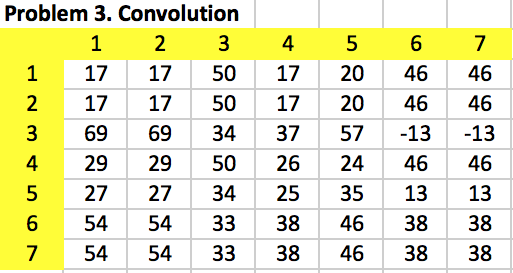
\includegraphics[width=80mm]{/Users/donj/workspace/cs585/Lab2/convolution.png}
\end{figure}

\item
These are the erosion and dilation of the original image:
\begin{figure}[H]
\centering
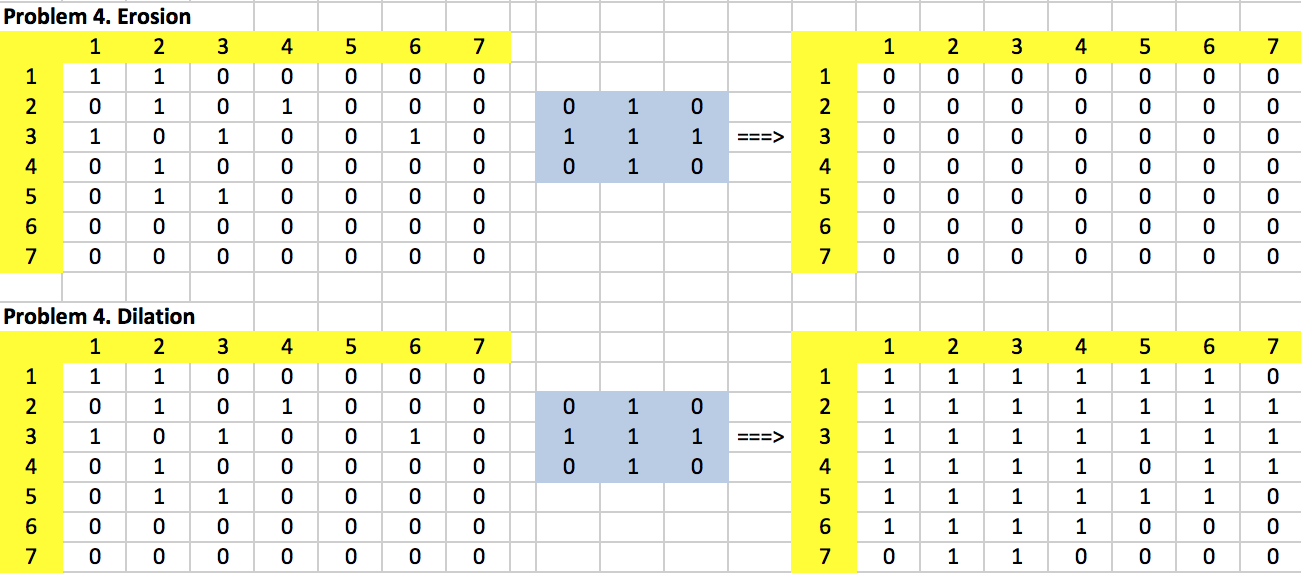
\includegraphics[width=140mm]{/Users/donj/workspace/cs585/Lab2/morphology.png}
\end{figure}

\section{Lecture preparation (3 points)}

\subsection{Preparation for Lecture 4}
Read Viola-Jones and Summed Area Table articles.

\subsection{Preparation for Lecture 5 (3 pts)}
In Lecture 5, we will discuss image pyramids for performing multi-scale feature
detection. Under the folder for Assignment 2, there is a folder called "camoEggsPyramid." Use your program from section 1.2 to perform edge detection on each of the images in the folder. What do you notice about the way the edge-finding and region-filling works on each of the images in the pyramid?

The most obvious thing is that the images get much smaller and more pixelated as you move up the levels. Also, it seams easier to detect complete edges as you move up the levels.

\end{enumerate}

\end{document}
